\section{Theorie}
\label{sec:Theorie}

% In knapper Form sind die physikalischen Grundlagen des Versuches, des Messverfahrens, sowie sämtliche für die Auswertung erforderlichen Gleichungen darzustellen. (Keine Herleitung)

% (eventuell die Aufgaben)

% Der Versuchsaufbau: Beschreibung des Versuchs und der Funktionsweise (mit Skizze/Bild/Foto)

Eine häufig verwendete Methode Röntgenstrahlung zu erzeugen ist die sogenannte Röntgenröhre.
Hier werden von einer Glühkathode Elektronen ausgesendet, welche im elektrischen Feld auf eine Anode hin beschleunigt werden.
Nun führen zwei Vorgänge zur Aussendung von Röntgenstrahlung.

Beim Ersten wird das Elektron durch das elektrische Feld der Elekronen im Anodenmaterial abgebremst.
Hierbei verliert das Elektron Energie, welche in From von Photonen ausgesendet wird.
Dieser Vorgang führt zum kontinuierlichen Spektrum, welches auch Bremsberg genannt wird und auf \autoref{fig:bremsberg} dargestellt ist.

\begin{figure}
    \centering
    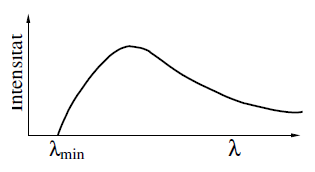
\includegraphics[width=0.5\textwidth]{images/bremsberg.png}
    \caption{Skizze des Bremsbergs bei Röntgenstrahlung.\cite{V602}}
    \label{fig:bremsberg}
\end{figure}

Der zweite Vorgang ist der Stoßprozess vom eintreffenden Elektron mit einem Elektron im Anodenatom.
Durch diesen Stoß wird ein Elektron aus einer der inneren Schalen aus dem Atom gelöst und hinterlässt eine Leerstelle.
Ein Elektron aus einer äußeren Schale wird nun die innere Schale besetzen und sendet hierbei ebenfalls ein Photon aus.
Dieses Photon hat gerade die Energie der Energiedifferenz der beiden Energieniveaus.
Durch die diskreten Energiedifferenzen ensteht somit ein diskretes Spektrum, welches als charakteristisches Spektrum bezeichnet wird.
Im charakteristischen Spektrum werden die einzelnen Linien mit Buchstaben wie $K_\alpha,K_\beta,L_\alpha,...$ bezeichnet.
Hier entspricht der Buchstabe der inneren Schale und das griechische Symbol der äußeren Schale.

Die Bindungsenergie auf der n-ten Schale $E_n$ hängt in einem Atom mit mehreren Elektronen unter Anderem von Abschirmeffekten des Kerns ab und kann mit
\begin{equation}
    E_n = -\frac{R_\infty(Z-\sigma)^2}{n^2}
\end{equation}
berechnet werden. 
$R_\infty=\SI{13.6}{\electronvolt}$ ist die Rydbergenergie, $Z$ die Ordnungszahl und $\sigma$ die Abschirmkonstante.\cite{V602}
Nach dem Moseley'schen Gesetz wird z.B die $K_\alpha$ Linie näherungsweise bei
\begin{equation}
    E_K = R_\infty(Z-\sigma)^2
    \label{eq:moseley}
\end{equation}
erwartet.
Allerdings führen weitere quantenmechanische Effekte wie z.B. der Spin zu Variationen dieser Bindungsenergie.
Dadurch sind die charakteristischen Linien noch detaillierter unterteilt und das Spektrum innerhalb einer Linie erscheind annähernd kontinuierlich.

\begin{figure}
    \centering
    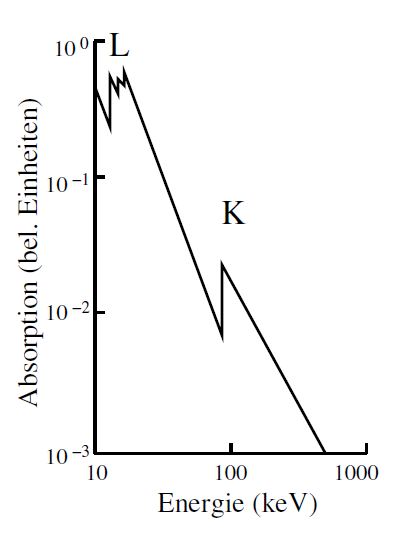
\includegraphics[width=0.4\textwidth]{images/absorption.png}
    \caption{Skizze des Absorptionsspektrums bei Röntgenstrahlung.\cite{V602}}
    \label{fig:absorption}
\end{figure}

Betrachtet man nun die Absorption von Röntgenstrahlung, fallen beim Absorptionskoeffizienten sprunghafte Anstiege trotz des generellen Abstiegs auf.(siehe \autoref{fig:absorption})
An diesen Stellen entspricht die Photonenenergie gerade der Bindungsenergie eines Elektrons und die Photonen können ab dieser Energie die Elektronen aus dem Atom lösen und somit wird das Photon absorbiert.
Die entsprechenen Absorptionsenergien werden je nach Schale $K$-,$L$-,...Kante genannt.
Wenn die Energie $E_K$ der $K$-Kante bekannt ist kann über die Sommerfeldsche Feinstrukturformel die Abschirmkonstante 
\begin{equation}
    \sigma_K = Z - \sqrt{\frac{E_K}{R_\infty}-\frac{\alpha^2Z^4}{4}}
    \label{eq:abschirm}
\end{equation}
berechnet werden. $\alpha=\num{7.297e-3}$ ist hier die Sommerfeldsche Feinstrukturkonstante.\cite{physics_constants}

In diesem Versuch wird das Röntgenspektrum mithilfe der Bragg'schen Reflexion bestimmt.
Hier wird die einfallende Strahlung an einem dreidimensionalen Gitter gebeugt und je nach Ein-/Ausfallswinkel tritt näherungsweise nur bei einer spezifische Wellenlänge konstruktive Interferenz auf. 
Wobei die Maximal Intensität bei einem Ausfallswinkel gleich dem Einfallswinkel erwartet wird.
Dies wird als Bragg Bedingung bezeichnet und der Versuch sollte so aufgebaut sein, dass diese Bedingung näherungsweise erfüllt ist.
Somit kann die Wellenlänge $\lambda$ zum Winkel $\theta$ über
\begin{equation}
    \lambda = \frac{2d}{n}\sin\theta
    \label{eq:bragg}
\end{equation}
bestimmt werden, wobei $n$ der Beugungsordnung entspricht.
Als 3 dimensionales Gitter wird hier ein LiF-Kristall mit einer Gitterkonstante $d=\SI{2.014e-12}{m}$ verwendet.
Außerdem wird nur die erste Beugungsordnung($n=1$) beachtet.

Aus der Wellenlänge der Strahlung lässt sich die Photonenenergie über
\begin{equation}
    E = \frac{hc}{\lambda}
    \label{eq:energie}
\end{equation}
bestimmen. 
$h=\SI{4.136e-15}{\electronvolt}$ ist das Plancksche Wirkungsquantum und $c=\SI{2.998e8}{\metre\per\second}$ ist die Lichtgeschwindigkeit.\cite{physics_constants}